\documentclass[12pt,a4paper]{article}
\usepackage[utf8]{inputenc}
\usepackage[T2A]{fontenc}  
\usepackage[russian]{babel}
\usepackage[left=3cm, right=1.5cm, top=2cm, bottom=2cm]{geometry}
\usepackage{amsmath}
\usepackage{amsfonts}
\usepackage{amssymb}
\usepackage{graphicx}
\usepackage{bm}
\usepackage{float}
\usepackage{hyperref}
\usepackage{booktabs}
\usepackage{array}
\usepackage{caption}

\begin{document}

\title{\textbf{Моделирование работы лазерного поляриметра на ускорительном комплексе ВЭПП-4М}}
\author{Эннс Сергей}
\date{\today}
\maketitle

\section*{Введение}

Одна из задач физики элементарных частиц состоит в изучении и дополнении
Стандартной модели, которая описывает, как взаимодействуют частицы во
Вселенной. Перед нами стоит задача нахождения массы $\Upsilon$(1S)-мезона; эта
частица представляет собой систему из b-кварка и b-антикварка. 

В лаборатории его получают столкновением электрона и позитрона. При их аннигиляции образуется виртуальный фотон, который с некоторой вероятностью превратится в $\Upsilon$-мезон. Если энергия виртуального фотона близка к его массе, происходит резонанс, и сечение рождения резко повышается. Перед лабораторией как раз стоит задача построения этой резонансной кривой, пик которой соответствует массе $\Upsilon$-мезона.

Для измерения энергии пучка используется метод резонансной деполяризации,
разработанный в ИЯФ. В его основе лежит прецизионное измерение частоты
прецессии спина, факт деполяризации регистрируется лазерным поляриметром,
работающем по принципу обратного комптоновского рассеяния.

Передо мной были поставлены следующие задачи:
\begin{itemize}
\item написание генератора комптоновского рассеяния;
\item проведение моделирования с учётом нового медного зеркала;
\item привести результаты моделирования к формату, который принимает программа подгонки для эксперимента;
\item проверить соответствие результатов работы программы обработки данных, используемой в реальном эксперименте по измерению массы $\Upsilon-$мезона с параметрами, закладываемыми при моделировании.
\end{itemize}
Моя работа по моделированию лазерного поляриметра позволит определить систематическую погрешность при подгонке поляризации электронов и будет полезной для улучшения измерения поляризации.
\section{Измерение энергии пучка}
\subsection*{Метод резонансной деполяризации} 
Электронный пучок в магнитном поле поляризуется посредством
синхротронного излучения, так как состояние со спином, направленным
антипараллельно полю обладает наименьшей энергией. Его спин прецессирует
с частотой
\begin{equation}
\Omega = \omega_{rev} \left(1 + \dfrac{E}{m_e c^2} \dfrac{\mu'}{\mu_0}\right)
\end{equation}

где $\omega_{rev}$ --- частота обращения пучка в ускорителе, E --- его энергия

При введении внешнего электромагнитного
поля с частотой $\omega_d$, удовлетворяющей условию
\begin{equation}
\Omega = n \omega_{rev} + \omega_d
\end{equation}

происходит деполяризация. Плавно меняя частоту колебаний в заданном
диапазоне, по моменту времени, когда произошло разрушение поляризации
пучка, мы определяем частоту деполяризатора в этот момент.

Деполяризация регистрируется лазерным поляриметром, который работает следующим образом: циркулярно поляризованные фотоны рассеиваются на ультрарелятивистских электронах, а детектор фиксирует их координаты. Если пучок поперечно поляризован, то мы увидим вертикальную
асимметрию.

\section{Моделирование комптоновского рассеяния}
\subsection{Качественный анализ формулы для сечения}
В этом подпункте рассматривается качественная связь между параметрами $P, Q, \beta$ и формой пятна рассеянных фотонов. 

\begin{itemize}
    \item $P$ --- поляризация электронного пучка;
    \item $Q$ --- линейная поляризация фотона лазера;
    \item $\beta$ --- угол поворота плоскости поляризации.
\end{itemize}

\begin{equation}
\begin{aligned}
 \dfrac{d\sigma}{d\Omega} = 2\gamma^2 r_e^2 
 \bigg[\frac{1}{1+\eta^2+\kappa}\bigg]^2 
 \bigg(
 2 
 &+ \frac{\kappa^2}{(1+\eta^2)(1+\eta^2+\kappa)}
 \\
 &- \frac{4\eta^2}{(1+\eta^2)^2}
 \big(1-Q\cos(2[\varphi - \beta])\big)
 \\
 &+ 2\kappa P V 
 \frac{\eta \sin \varphi}{(1+\eta^2)(1+\eta^2+ \kappa)}
 \bigg)
\end{aligned}
\end{equation}

В выражении выделяются три компоненты. Обозначим их $S_0$, $S_Q$ и $S_{PV}$ соответственно.

\medskip
\textbf{1. Неполяризационный вклад $S_0$}

Этот член не зависит от азимутального угла $\varphi$ и формирует изотропный фон. Он определяет общий радиальный профиль пятна и его круговую симметрию.

\begin{figure}[H]
    \centering
    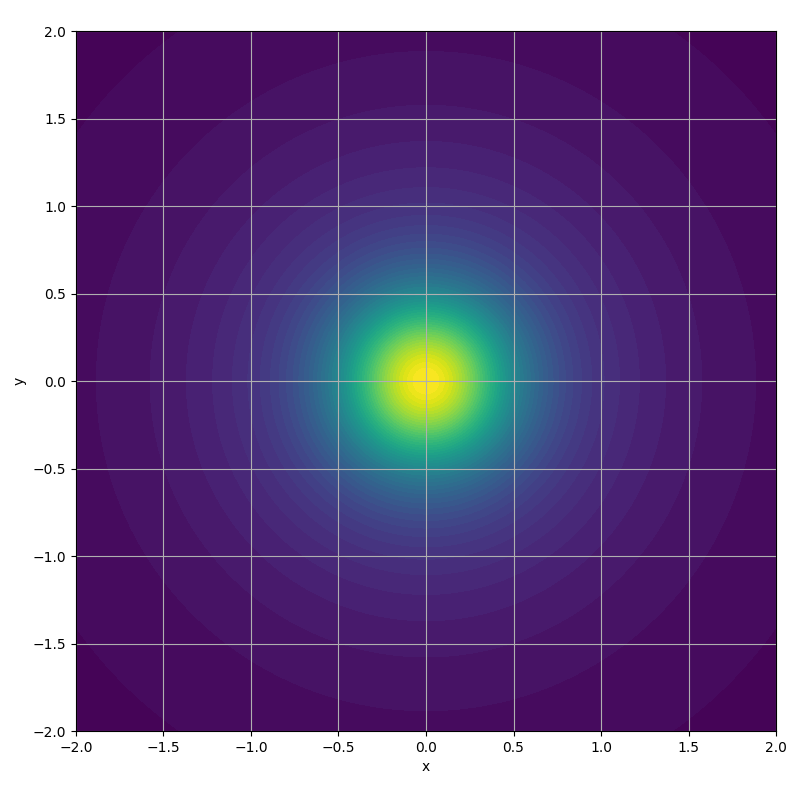
\includegraphics[width=0.5\linewidth]{pictures/Figure_100.png}
\end{figure}

\medskip
\textbf{2. Линейная поляризация: квадрупольный вклад $S_Q$}

Член, пропорциональный $Q$, содержит $\cos 2(\varphi - \beta)$ и порождает квадрупольную симметрию: четырёхлепестковую фигуру, повернутую на угол $\beta$. При разности распределений 
\[
\dfrac{d\sigma}{d\Omega}(Q) - \dfrac{d\sigma}{d\Omega}(-Q)
\]
изотропная часть исчезает, остаётся чистая квадрупольная картина.

\begin{figure}[H]
\centering
\begin{minipage}{0.45\linewidth}
\centering
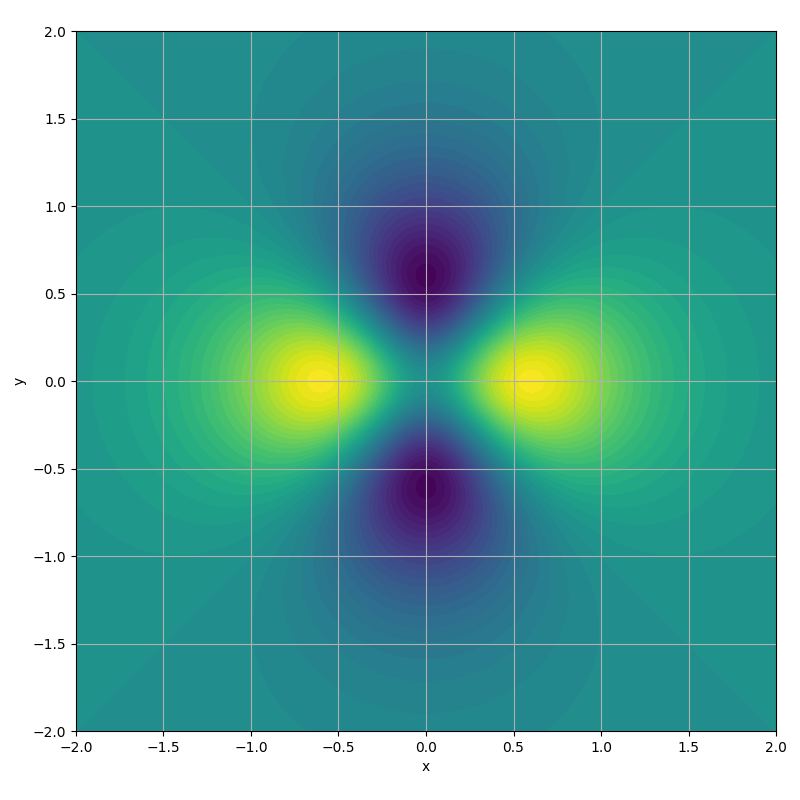
\includegraphics[width=\linewidth]{pictures/квадр 0.png}
\caption{$\beta = 0$}
\end{minipage}
\hfill
\begin{minipage}{0.45\linewidth}
\centering
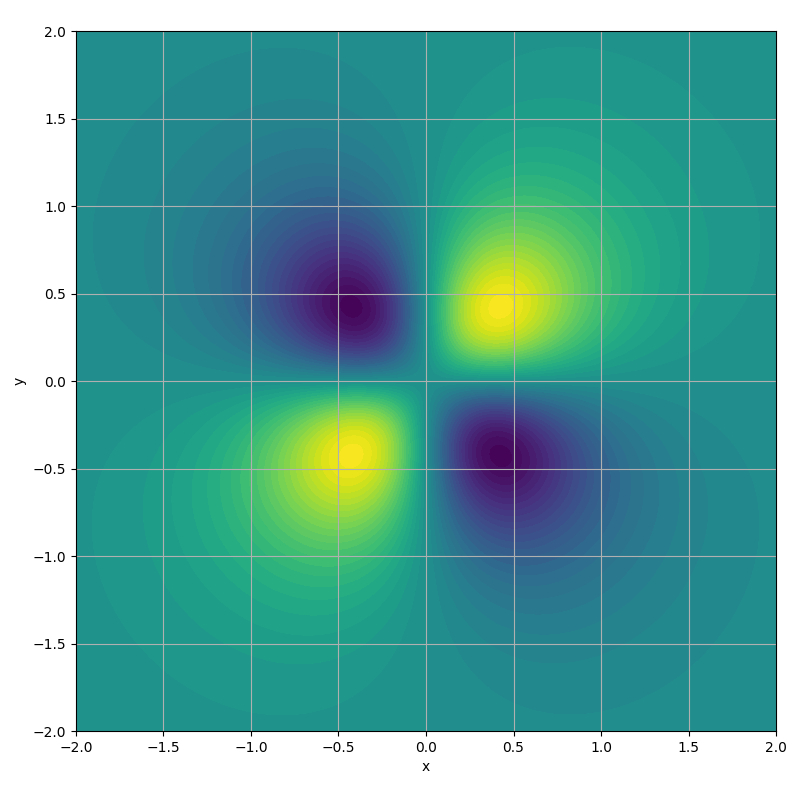
\includegraphics[width=\linewidth]{pictures/квадрi4.png}
\caption{$\beta = \pi/4$}
\end{minipage}
\end{figure}

\begin{figure}[H]
\centering
\begin{minipage}{0.45\linewidth}
\centering
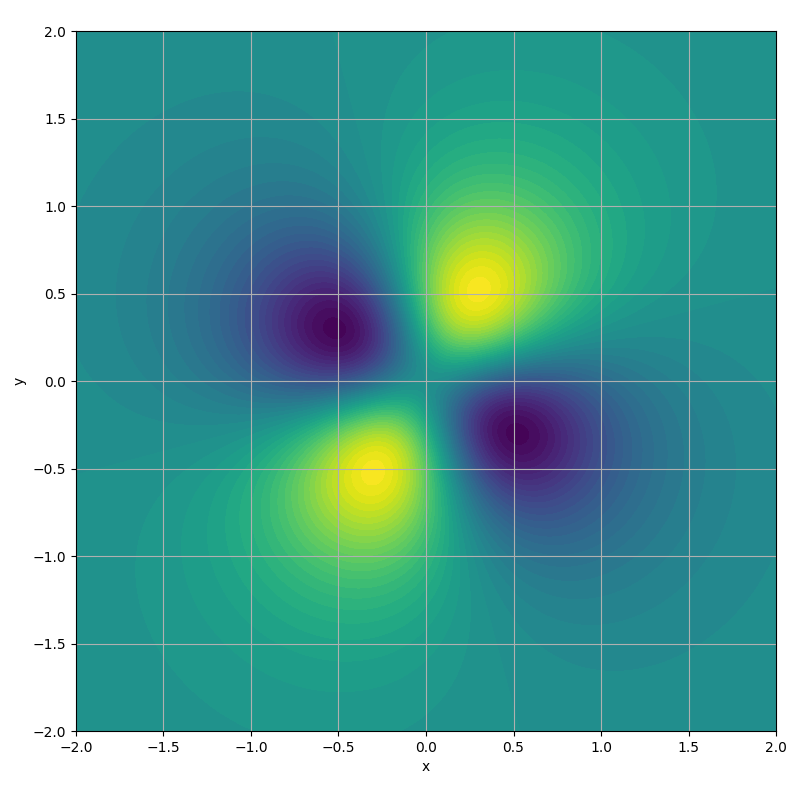
\includegraphics[width=\linewidth]{pictures/квадрпи3.png}
\caption{$\beta = \pi/3$}
\end{minipage}
\hfill
\begin{minipage}{0.45\linewidth}
\centering
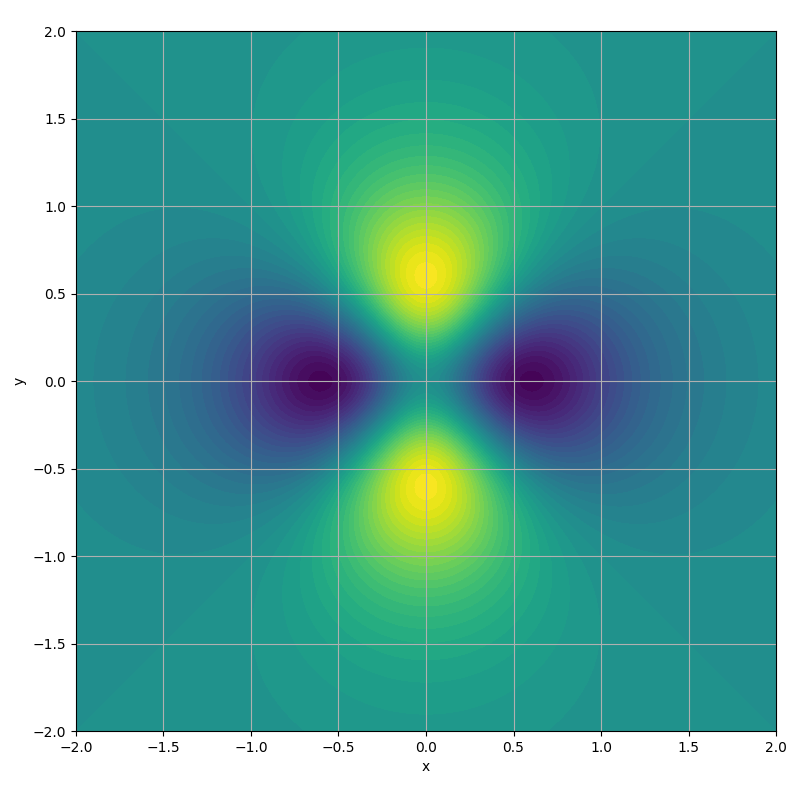
\includegraphics[width=\linewidth]{pictures/квадрпи2.png}
\caption{$\beta = \pi/2$}
\end{minipage}
\end{figure}

\medskip
\textbf{3. Круговая поляризация: дипольный вклад $S_{PV}$}

Член $S_{PV}$ содержит $\sin\varphi$ и даёт дипольную двухлепестковую структуру. Она проявляется только при $PV \neq 0$ и формирует вертикальную асимметрию.

\begin{figure}[H]
    \centering
    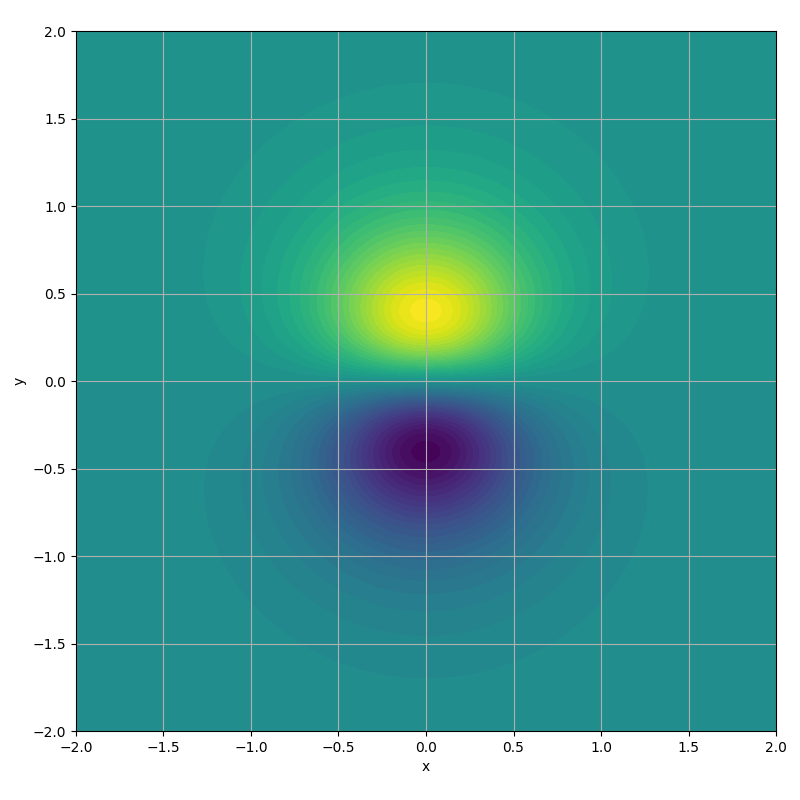
\includegraphics[width=0.45\linewidth]{pictures/дип.png}
\end{figure}

\medskip
\textbf{4. Пример комбинированного вклада}

Пусть $P = 0.6$, $Q = 0.5$, $\beta = \pi/6$.  

Суммарная форма пятна --- результат наложения изотропного фона, квадруполя и диполя.

\begin{figure}[H]
    \centering
    \begin{minipage}{0.22\linewidth}
        \centering
        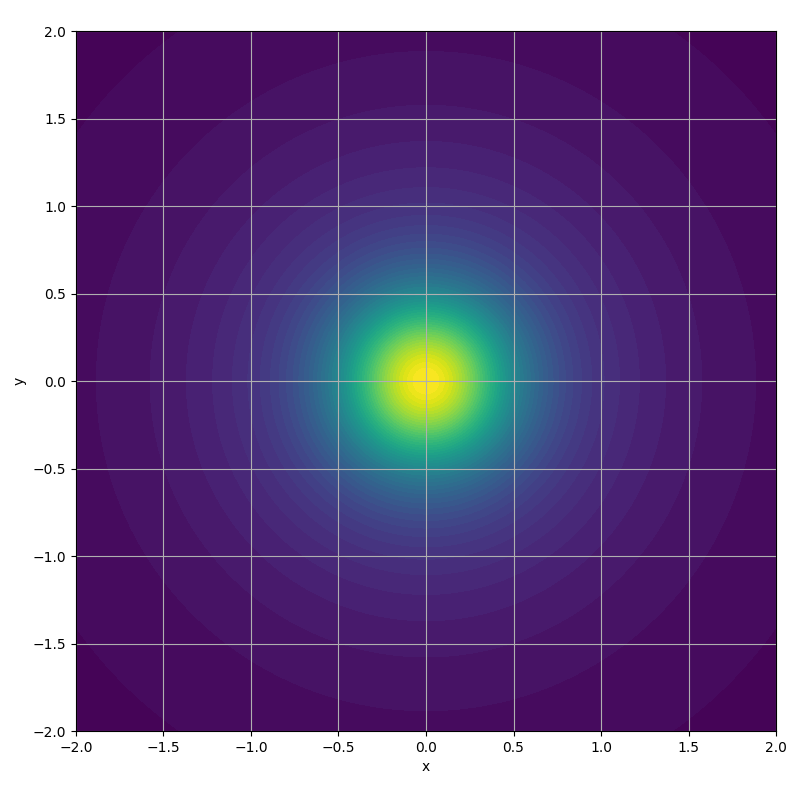
\includegraphics[width=\linewidth]{pictures/nw1.png}
    \end{minipage}
    \hfill
    \Large{$+$}
    \hfill
    \begin{minipage}{0.22\linewidth}
        \centering
        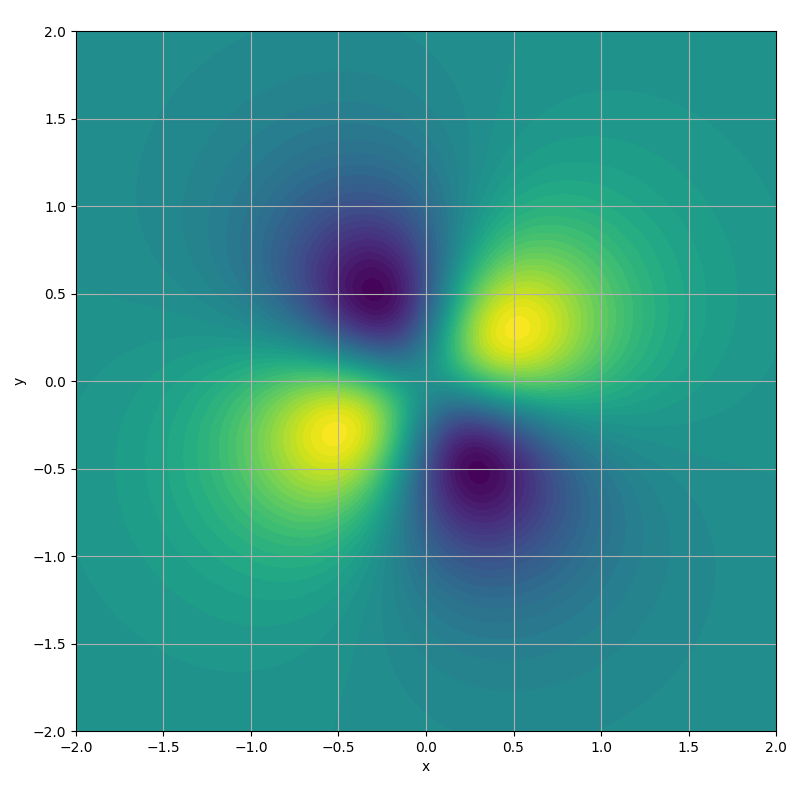
\includegraphics[width=\linewidth]{pictures/new2.png}
    \end{minipage}
    \hfill
    \Large{$+$}
    \hfill
    \begin{minipage}{0.22\linewidth}
        \centering
        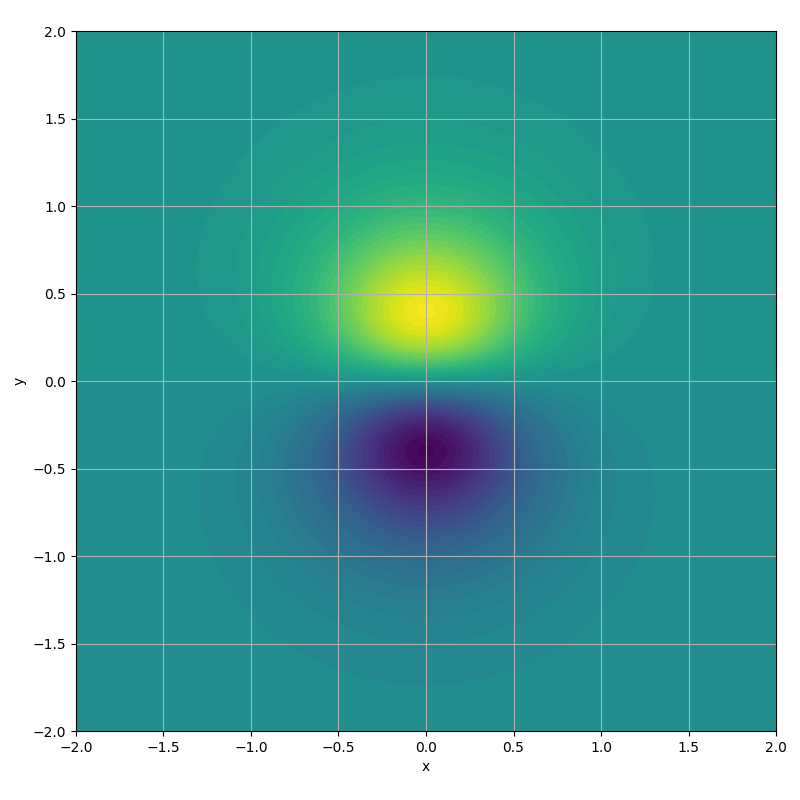
\includegraphics[width=\linewidth]{pictures/nw3.png}
    \end{minipage}
    \hfill
    \Large{$=$}
    \hfill
    \begin{minipage}{0.22\linewidth}
        \centering
        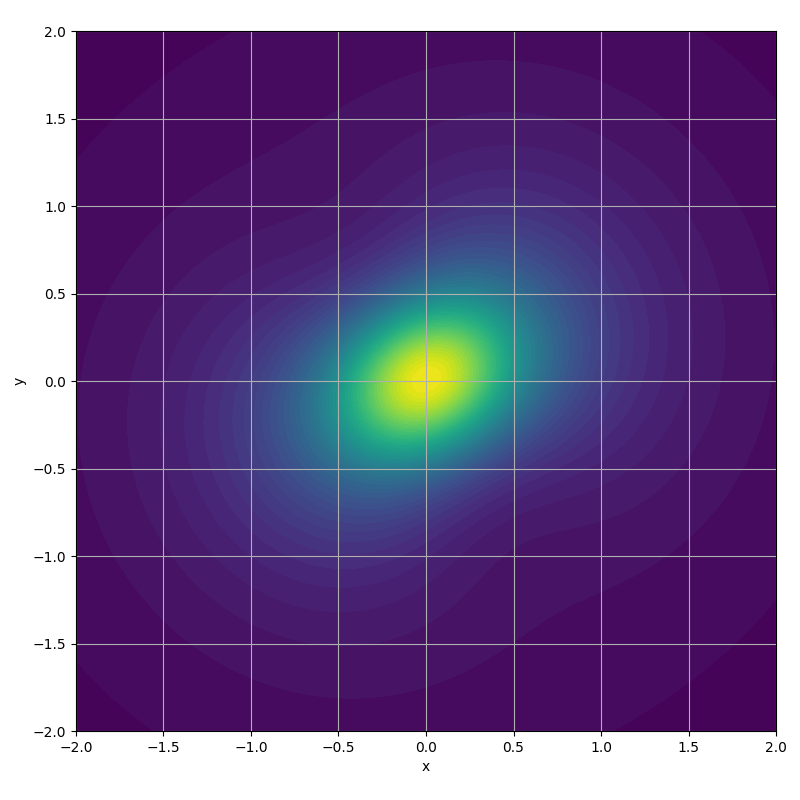
\includegraphics[width=\linewidth]{pictures/dfsdfdjfpiz.png}
    \end{minipage}
\end{figure}

\subsection{Моделирование углов рассеяния}
\subsubsection{Оптимизированный метод Неймана}
Дифференциальное сечение комптоновского рассеяния описывается формулой:
\begin{equation}
\label{eq:cross_section}
\begin{aligned}
\frac{d\sigma}{d\Omega}(\eta, \varphi) &= 2\gamma^{2}r_{e}^{2}
\left[\frac{1}{1+\eta^{2}+\kappa}\right]^{2} \times{} \\
&\quad \times \left(2 + \frac{\kappa^{2}}{(1+\eta^{2})(1+\eta^{2}+\kappa)} 
- \frac{4\eta^{2}}{(1+\eta^2)^{2}}\bigl(1-Q\cos (2[\varphi-\beta])\bigr)\right) + \\
&\quad + 4\gamma^{2}r_{e}^{2}\, PV\, \kappa \frac{\eta\sin\varphi}{(1+\eta^{2})(1+\eta^{2}+\kappa)^{3}}.
\end{aligned}
\end{equation}


Запишем функцию распределения с точностью до константы:
\begin{equation}
\label{eq:density_function}
\begin{aligned}
f(\eta, \varphi) = \frac{C}{\left(1 + \eta^2 + \kappa\right)^2} \Biggl(1 
&+ \frac{\frac{1}{2} \kappa^2}{(1+\eta^2)(1+\eta^2+\kappa)} \\
&- \frac{2\eta^2}{(1+\eta^2)^2}\bigl(1-Q\cos (2[\varphi-\beta])\bigr) \\
&+ \kappa\, PV\, \frac{\eta \sin \varphi}{(1+\eta^2)(1+\eta^2+\kappa)} \Biggr).
\end{aligned}
\end{equation}


Прямое применение метода Неймана к $f(\eta,\varphi)$ неэффективно при больших $\eta$, 
так как плотность по полярному углу быстро убывает как $\sim 1/\eta^3$, и большинство попыток отвергается.

Чтобы ускорить генерацию, выделим из $f(\eta,\varphi)$ множитель, который точно 
интегрируется и хорошо аппроксимирует поведение плотности в хвостах. 
Можно записать в следующей форме:
\begin{equation}
dF = f(\eta, \varphi)\,\eta\, d\eta\, d\varphi = C\,\frac{\eta\, d\eta\, d\varphi}{(1+\eta^2+\kappa)^2}\, B(\eta, \varphi),
\end{equation}
где
\begin{equation}
B(\eta,\varphi) = 1 + \frac{\frac{1}{2}\kappa^2}{(1+\eta^2)(1+\eta^2+\kappa)} 
- \frac{2\eta^2}{(1+\eta^2)^2}\bigl(1-Q\cos(2[\varphi-\beta])\bigr) 
+ \kappa\, PV\, \frac{\eta\sin\varphi}{(1+\eta^2)(1+\eta^2+\kappa)}.
\end{equation}
При больших значениях угла вклад $B(\eta, \varphi)$ ничтожен.

Делаем замену $f(\eta, \varphi)\eta\, d\eta = dG$:
\begin{equation}
dF = B(\eta, \varphi)\, dG\, d\varphi.
\end{equation}

Интегрируя $dG$, получаем:
\begin{equation}
G(\eta) = \int_0^\eta C\,\frac{\eta' d\eta'}{(1+\eta'^2+\kappa)^2} 
= \frac{C\eta^2}{2(1+\kappa)(1+\eta^2+\kappa)}.
\end{equation}

Нормировка:
\begin{equation}
\lim_{\eta \to \infty} G(\eta) = \lim_{\eta \to \infty} 
\frac{C}{2(1+\kappa)\left(1 + \frac{1+\kappa}{\eta^2}\right)} 
= \frac{C}{2(1+\kappa)} = 1 \quad\Rightarrow\quad C = 2(1+\kappa).
\end{equation}

Таким образом,
\begin{equation}
G(\eta) = \frac{\eta^2}{1 + \eta^2 + \kappa}.
\end{equation}

Слишком большие углы можно не учитывать. Положим $\eta_{\text{max}} = 10$, что покрывает $99\%$ событий.

Случайную величину $\eta$ получаем из условия $G \sim U\!\left(0,\ \dfrac{\eta_{\text{max}}^2}{1+\eta_{\text{max}}^2+\kappa}\right)$:
\begin{equation}
\eta = \sqrt{\frac{(1+\kappa)G}{1-G}}.
\end{equation}

\textbf{Алгоритм}
\begin{enumerate}
    \item Генерируем $\eta$ из огибающей согласно формуле выше.
    \item Выбираем угол $\varphi$ равномерно на $[0, 2\pi)$.
    \item Вычисляем значение скобки $B(\eta,\varphi)$.
    \item Принимаем пару $(\eta,\varphi)$, если случайная величина 
          $u \in [0, B_{\text{max}}]$ удовлетворяет условию $u \le B(\eta,\varphi)$ 
          (метод Неймана). Иначе повторяем сначала.
\end{enumerate}


\subsubsection{Проверка моделирования}


Для проверки подгоним параметры распределения, используя смоделированные этим алгоритмом углы. Для этого подойдет метод максимального правдоподобия.

Разобьем пространство углов на $N$ ячеек. Количество событий в каждой ячейке подчиняется распределению Пуассона.

Вероятность $n_i$ событий в $i$-й ячейке равна:
\begin{equation}
P_i(n_i) = \dfrac{\mu_i^{n_i}e^{-\mu_i}}{n_i!}
\end{equation}

Функция правдоподобия:
\begin{equation}
\ln L\left(P,Q,\beta \right) = \sum_{i=1}^N \left[-\mu_i + n_i \ln(\mu_i) - \ln(n_i!) \right].
\end{equation}
Найдя максимум этой функции, возможно оценить параметры распределения $P^*, Q^*, \beta^*$.

Количество событий -- $10^6$

Гистограммы:

\begin{figure}[H]
    \centering
    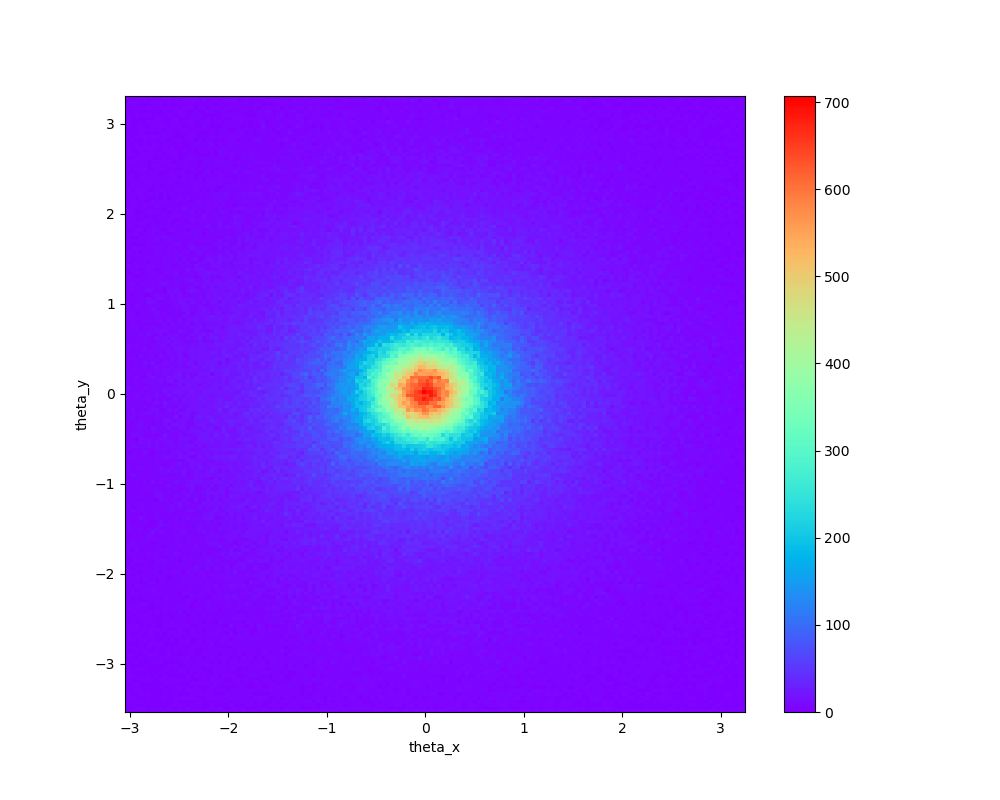
\includegraphics[width=0.7\linewidth]{pictures/Fig_1_0_0.png}
    \caption{$P=1; Q=0; \beta=0.$}
    \label{fig:placeholder}
\end{figure}

\begin{figure}[H]
    \centering
    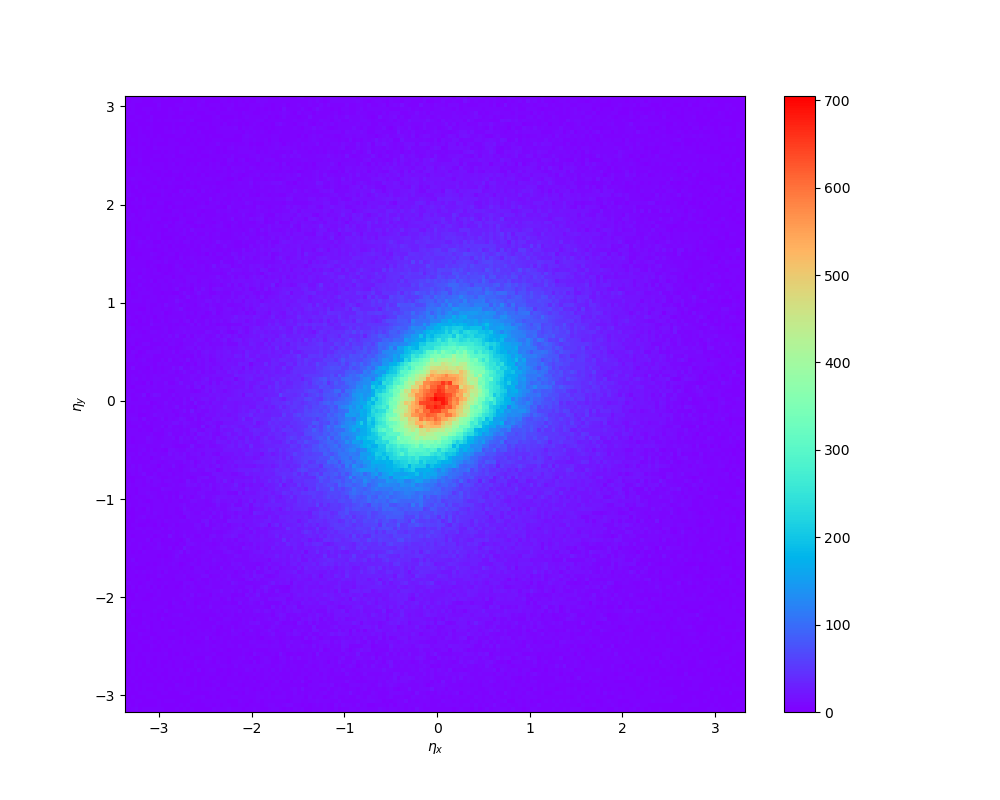
\includegraphics[width=0.7\linewidth]{pictures/Fig_1_0-5_0-7.png}
    \caption{$P=1; Q=0,5; \beta=0,7.$}
    \label{fig:placeholder}
\end{figure}

\begin{figure}[H]
    \centering
    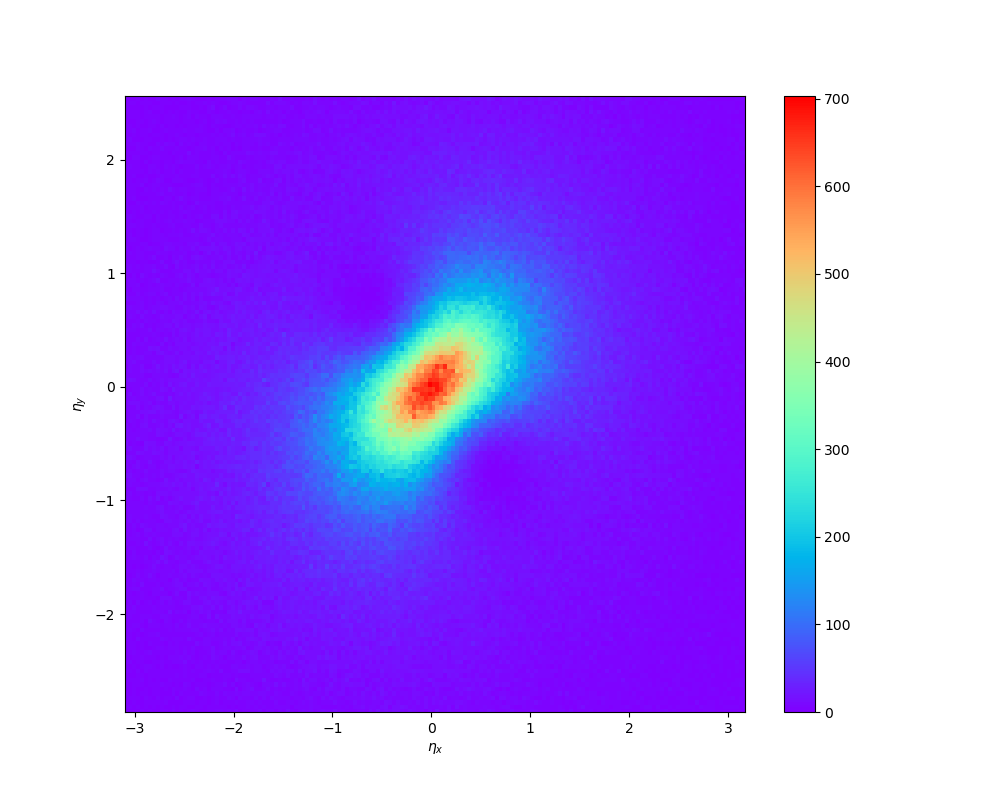
\includegraphics[width=0.75\linewidth]{pictures/figg.png}
    \caption{$P=1; Q=1; \beta=0,7.$}
    \label{fig:placeholder}
\end{figure}

\begin{table}[H]
\centering
\caption{Результаты восстановления параметров}
\begin{tabular}{lccc}
\toprule
Параметр & Истинное значение & Восстановленное значение & Отклонение \\
\midrule
$P$ & 1 & $1,00 \pm 0,06 $& $0$\\
$Q$ & 0 & $0,0042 \pm 0,0024$ & $1,75 \sigma$ \\
$\beta$ (рад) & 0 & $2,42 \pm 0,28$ & $8,64 \sigma$ \\
\bottomrule
$P$ & 1 & $ 1,00 \pm 0,01 $&  0\\
$Q$ & 0,5 & $ 0,4992 \pm 0,0022$ &  $0,36 \sigma$\\
$\beta$ (рад) & 0,7 & $ 0,6979 \pm 0,0023 $ & $0,91 \sigma$ \\
\bottomrule
$P$ & 1 & $ 0,34 \pm 0,22 $&  $3\sigma$\\
$Q$ & 1 & $ 0,9972 \pm 0,0012$ &  $2,3 \sigma$\\
$\beta$ (рад) & 0,7 & $ 0,6998 \pm 0,0010 $ & $0,2 \sigma$ \\
\bottomrule
\end{tabular}
\end{table}

Графики (синий -- моделирование, красный -- подгонка):
\begin{figure}[H]
    \centering
    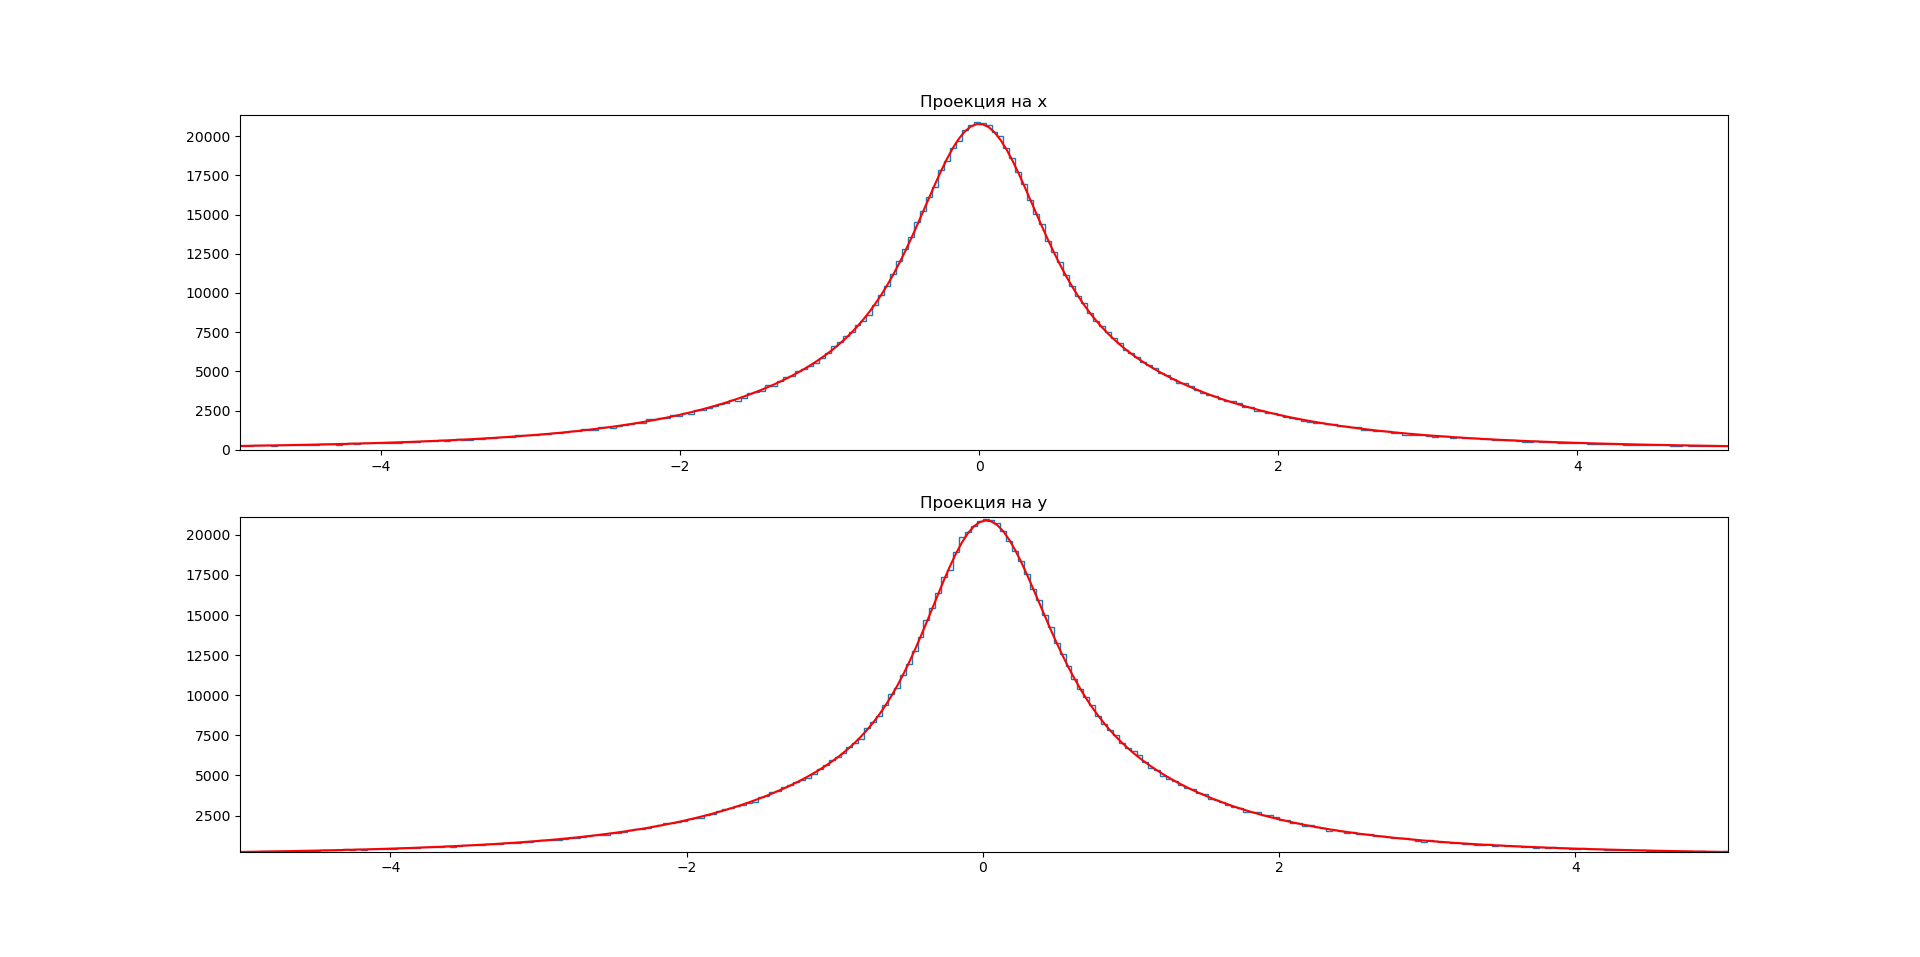
\includegraphics[width=1.\linewidth]{pictures/fit_1_0_0.png}
    \caption{$P=1; Q=0; \beta=0.$}
    \label{fig:placeholder}
\end{figure}

\begin{figure}[H]
    \centering
    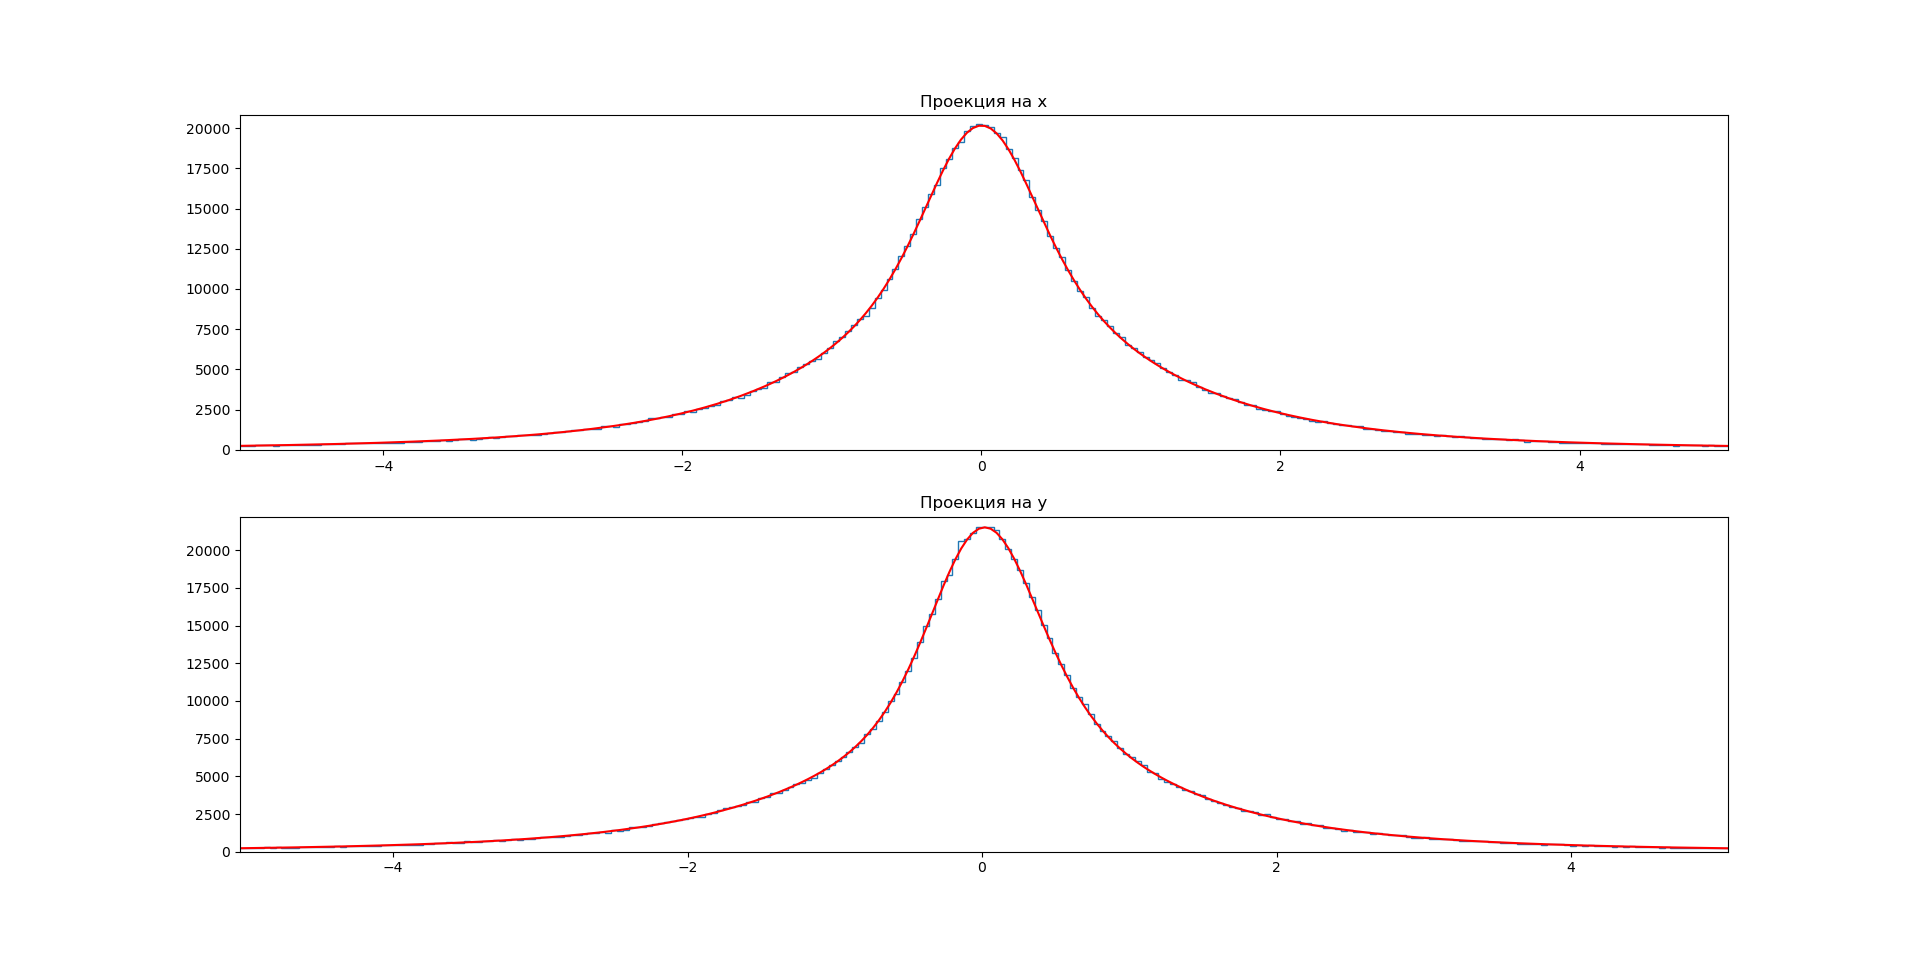
\includegraphics[width=1.\linewidth]{pictures/fit_1_0-5_0-7.png}
    \caption{$P=1; Q=0,5; \beta=0,7.$}
    \label{fig:placeholder}
\end{figure}

\begin{figure}[H]
    \centering
    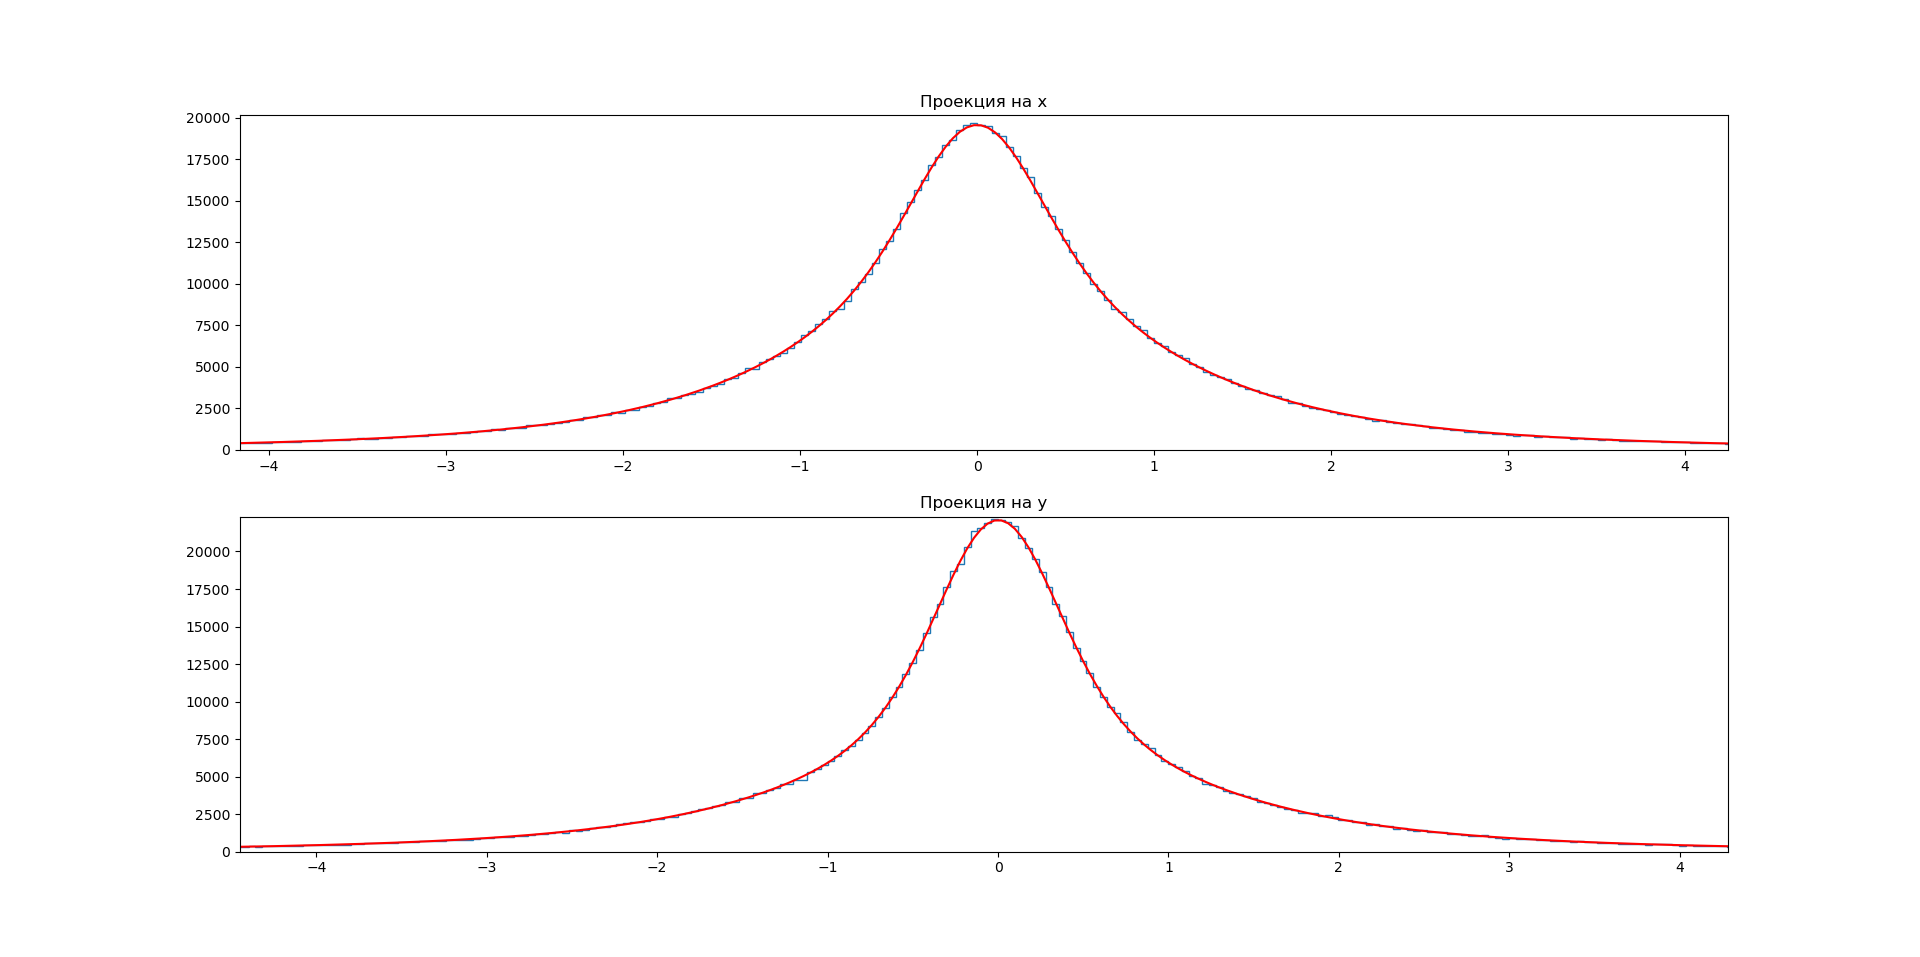
\includegraphics[width=1.\linewidth]{pictures/fittt.png}
    \caption{$P=1; Q=1; \beta=0,7.$}
    \label{fig:placeholder}
\end{figure}

Мы можем сделать вывод, что подгонка подтвердила правильность генератора, что видно во второй строке таблицы 1. Я специально привёл примеры плохой подгонки при неподходящих параметрах (1 и 3 строки) для понимания границ применимости. В первом случае линейная поляризация отсутствует и, соответственно, угол поворота линейной поляризации неопределён и не может быть подогнан. Третий случай аналогичен: если поляризация полностью линейна, то круговая отсутствует. То есть слагаемое с $P$ занулено, что делает невозможным его точную подгонку.

\subsection{Рассеяние на электронном пучке}

\subsubsection{Преобразования для углов}
Ось Z направим против движения первичного фотона. Обозначим $\vartheta - $ угол отклонения направления электрона от оси Z, $\theta - $ угол рассеяния фотона на электроне. Тогда $\alpha_1 = \pi - \vartheta$, $\alpha_2 = \theta$, а $\alpha_3 = \pi - \delta$, где $\delta-$ угол отклонения рассеянного фотона от оси Z, который мы вычислим ниже. Электроны релятивистские, значит, углы малы и мы можем рассматривать угловые отклонения от оси как векторы на касательной к сфере плоскости в точке её пересечения с этой осью. Базис -- декартовы орты.

\begin{equation}
    \bm{\tau}_e = 
    \begin{pmatrix}
        \vartheta \cos \phi \\
        \vartheta \sin \phi
    \end{pmatrix} - \text{вектор угла отклонения электрона}
\end{equation}

\begin{equation}
    \bm{\tau}_{\gamma} = 
    \begin{pmatrix}
        \theta \cos (\varphi + \phi) \\
        \theta \sin (\varphi + \phi)
    \end{pmatrix} - \text{вектор угла рассеяния фотона}
\end{equation}
Для вектора отклонения фотона имеем
\begin{equation}
    \bm{\delta} =  \bm{\tau}_{\gamma} + \bm{\tau}_e = 
    \begin{pmatrix}
         \vartheta \cos \phi +  \theta \cos (\varphi + \phi) \\
         \vartheta \sin \phi +  \theta \sin (\varphi + \phi)
    \end{pmatrix}
\end{equation}
А его длина равна
\begin{equation}
    \delta^2 = \theta^2 + \vartheta^2 + 2\theta\vartheta\cos\varphi
\end{equation}
Итак, угол между фотонами:
\begin{equation}
    \alpha_3 = \pi - \sqrt{\theta^2 + \vartheta^2 + 2\theta\vartheta\cos\varphi}
\end{equation}


\subsubsection{Энергия рассеянных фотонов}
Четырёхимпульсы
\begin{itemize}
\item $P_{\gamma0} $ -- начального фотона;
\item $P_{\gamma} $ -- рассеянного фотона;
\item $P_{e0} $ -- электрона до столкновения;
\item $P_{e} $ -- электрона после столкновения.
\end{itemize}




\bigskip
Закон сохранения четырёхимпульса:

\begin{equation}
    P_{\gamma0} + P_{e0} = P_{\gamma} + P_{e}
\end{equation}

Инвариантная запись 
\begin{equation}
    (P_{\gamma0} + P_{e0} - P_{\gamma})^2  = P^2_{e}
\end{equation}

Раскрыв скобки, получаем

\begin{equation}
   P_{e0}P_{\gamma0} - P_{e0}P_{\gamma} - P_{\gamma0}P_{\gamma}  = 0
\end{equation}

Обозначим \\
угол между начальным фотоном и электроном -- $\alpha_1$;  \\
угол между рассеянным фотоном и электроном -- $\alpha_2$; \\
угол между фотонами -- $\alpha_3$. \\
И переобозначим временные компоненты векторов $P^0_{e0} = \varepsilon$, $P^0_{\gamma0} = \omega$, $P^0_{\gamma} = \omega'$.
\begin{equation}
    \omega \varepsilon - \varepsilon \beta \omega \cos \alpha_1 - \varepsilon\omega' + \omega' \varepsilon \beta \cos \alpha_2 - \omega \omega' + \omega\omega' \cos \alpha_3 = 0
\end{equation}

Итак, для энергии рассеянного фотона получаем

\begin{equation}
    \omega' = \omega \dfrac{1 - \beta\cos\alpha_1 }{1 - \beta \cos\alpha_2 + \dfrac{\omega}{\varepsilon}\left(1-\cos\alpha_3 \right)}
\end{equation}



Теперь мы можем подставить сгенерированные углы рассеяния фотонов и разброса электронов в формулу (19) для получения корректного распределения по энергиям.
\begin{equation}
    \omega' = \omega \dfrac{1 + \beta\cos\vartheta  }{1 - \beta \cos\theta + \dfrac{\omega}{\varepsilon}\left(1+\cos\sqrt{\theta^2 + \vartheta^2 + 2\theta\vartheta\cos\varphi}\right)}
\end{equation}
Разложим косинусы до второго порядка
\begin{equation}
    \omega' = \omega \dfrac{1+\beta \left(1 - \dfrac{\vartheta^2}{2}  \right)}{1 - \beta \left( 1 - \dfrac{\theta^2}{2} \right) + \dfrac{\omega}{\varepsilon}\left(2 + \theta\vartheta\cos\varphi+\dfrac{\theta^2 + \vartheta^2 }{2}\right)}
\end{equation}

Используем ультрарелятивистское приближение $\beta = 1 - \dfrac{1}{2\gamma^2} + o(1/\gamma^2)$
\begin{equation}
    \omega' = \omega \dfrac{2 - \dfrac{\vartheta^2}{2} }{\left(\dfrac{\theta^2}{2} + \dfrac{1}{2\gamma^2} \right) + \dfrac{\omega}{\varepsilon}\left(2 + \theta\vartheta\cos\varphi+\dfrac{\theta^2 + \vartheta^2 }{2}\right)}
\end{equation}

\subsubsection{Обновлённый алгоритм}
\begin{enumerate}
    \item Генерируем $\eta$ из огибающей согласно формуле выше.
    \item Выбираем угол $\varphi$ равномерно на $[0, 2\pi)$.
    \item Вычисляем значение скобки $B(\eta,\varphi)$.
    \item Принимаем пару $(\eta,\varphi)$, если случайная величина 
          $u \in [0, B_{\text{max}}]$ удовлетворяет условию $u \le B(\eta,\varphi)$ 
          (метод Неймана). Иначе повторяем сначала.
    \item Генерируем координаты электрона по гауссу.
    \item Генерируем разброс электрона по гауссу.
    \item Складываем углы по формуле 17.
    \item Вычисляем энергию
    \item Запускаем фотон с заданными координатами, углами и энергией.
\end{enumerate}

\section{Моделирование в Geant4}

В этом разделе будет проделано моделирование прохождения рассеянных жёстких фотонов через экспериментальную установку.
\subsection{Геометрия установки}
Установка включает в себя следующие ключевые элементы:
\begin{itemize}
\item \textbf{Фланец вакуумной трубы}: диаметр --- 40 мм, толщина --- 1,5 мм.
\item \textbf{Зеркало:} диаметр --- 100 мм, толщина медного зеркала --- 4 мм, толщина водного слоя --- 17 мм, толщина стальных стенок (по обе стороны водного слоя) --- 1 мм.
\item \textbf{Конвертер:} материал --- свинец, толщина --- 20 мм (в реальности --- 12 мм), ширина --- 161,4 мм, высота --- 50,35 мм. Расположен на расстоянии 29,9 м от области взаимодействия лазера с пучком.
\item \textbf{Упрощённая модель детектора:} на данном этапе представлена тонким слоем аргона, регистрирующим координаты (x, y) заряженных частиц. Полноценная модель ГЭУ с падами и лавинным умножением будет реализована на следующем этапе.

\end{itemize}
\begin{figure}[H]
\centering
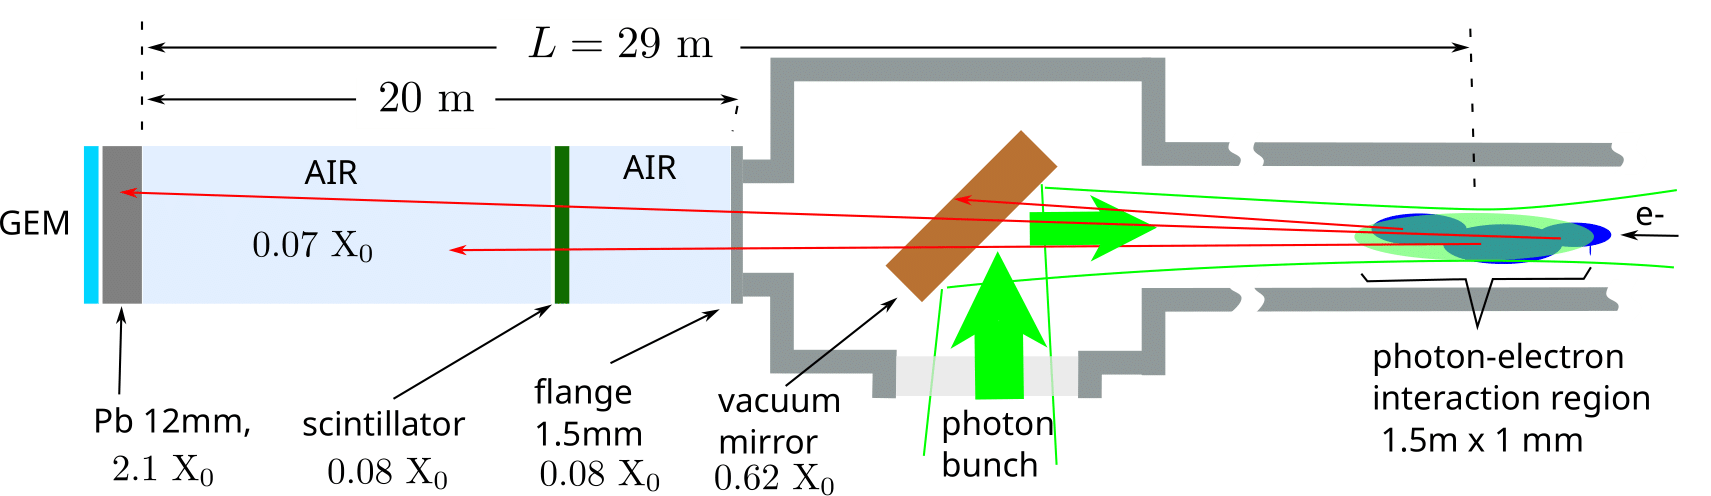
\includegraphics[scale=0.7]{pictures/material_scheme-1.png}
\caption{Схематичное изображение установки.}
\end{figure}

\subsection{Реализация физики}
Для моделирования взаимодействия частиц с элементами установки используется пакет Geant4. При создании пушки частиц с правильным распределением по углам рассеяния используется ранее написанный генератор комптоновского рассеяния. 

Для корректной реализации всех электромагнитных процессов, в основном --- ливней в конвертере, в Geant4 выбран список физики для электромагнетизма. Он включает:
\begin{itemize}
\item Для фотонов: фотоэффект, комптоновское рассеяние, рождение пар.
\item Для электронов/позитронов: ионизационные потери, тормозное излучение, множественное рассеяние.
\begin{figure}[H]
\centering
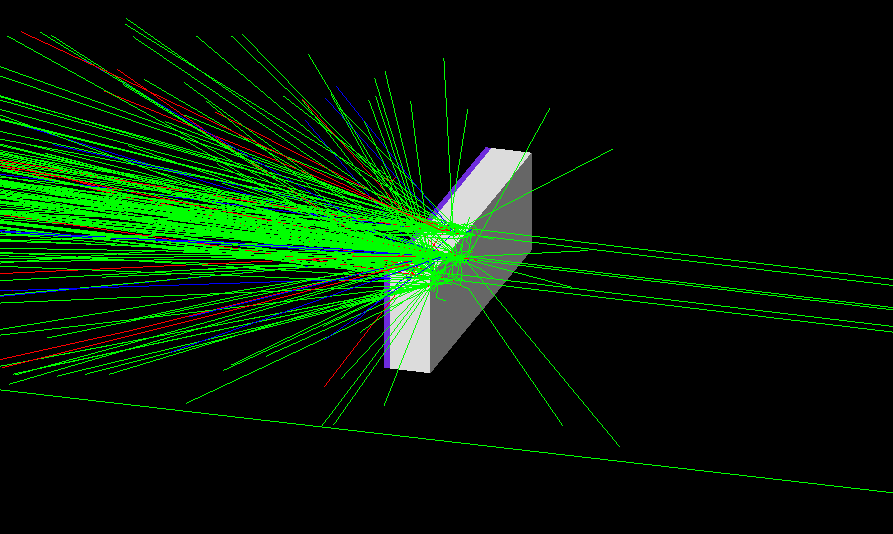
\includegraphics[scale=0.4]{pictures/rain.png}
\caption{Ливень в конвертере.}
\end{figure}
\end{itemize}

Из графика [позже вставлю график для сечений разных процессов] видно, что сечения различных электромагнитных процессов для фотона в веществе зависят от его энергии. Мы видим, что рождение пар и фотоэффект имеют порог реакции. Для фотоэффекта это необходимая энергия для ионизации электрона, то есть он равен энергии связи внешнего электрона в атоме. Для рождения пар порог обусловлен законами сохранения, найдём его.
\begin{equation}
    \gamma + Z \rightarrow e^+ + e^- + Z
\end{equation}
Воспользуемся инвариантностью квадрата суммарного четырёхимпульса системы. 
Инвариант до реакции
\begin{equation}
    inv = \left(\omega + M \right)^2 - \omega^2,
\end{equation} где $M -$ масса ядра.

Мы хотим найти порог реакции, то есть минимальную энергию фотона, при которой она возможна. В этом случае вся энергия уйдёт только на образование пары, без добавления кинетической энергии. Имнвариант после реакции равен квадрату суммы масс её продуктов.

Приравняем инварианту до реакции и получим

\begin{equation}
    \left(\omega_{min} + M \right)^2 - \omega_{min}^2 = \left( M + 2m_e \right)^2
\end{equation}

Разрешая уравнение относительно $\omega_{min}$, находим порог

\begin{equation}
    \omega_{min} = 2m_e\left(1+\dfrac{m_e}{M}\right)
\end{equation}
\\

Можно приближённо записать $\omega_{min} \approx 2m_e$, порог реакции примерно равен сумме масс электрона и позитрона (около 1 МэВ).


Конвертер нужен для превращения фотонов в электрон-позитронные пары, которые проще детектировать. Как мы видим, для энергии в 800 МэВ рождение пар сильно преобладает над другими процессами, что оправдывает использование конвертера. Эффективность конвертера тем выше, чем сильнее фотоны взаимодействуют с металлом. Посмотрим как зависит вероятность взаимодействия от толщины для разных металлов. 

Для этого проведём следующее моделирование в Geant4: разместим конвертер заданной толщины и материала на пути к фотонам и будем считать количество провзаимодействовавших с ним. 
Ниже приведена таблица, в которой отражена зависимость числа провзаимодействовавших фотонов от толщины разных металлов.
\\
Количество налетающих фотонов -- 100 000.
\begin{table}[h]
\centering
\begin{tabular}{|l|l|l|l|l|l|}
\hline
 & \multicolumn{5}{c|}{N} \\ \hline
$d,$ мм & W & Pb & U & Os & Au \\ \hline
 2& 34 302& 23 058& 36 896& 39 158& 35 706\\ \hline
 4& 56 779& 40 776& 60 225& 63 003& 58 501\\ \hline
 6& 71 455& 54 305& 74 687& 77 590& 73 471\\ \hline
 8& 81 448& 64 871& 84 038& 86 293& 82 606\\ \hline
 10& 87 762& 73 116& 90 096& 91 692& 88 639\\ \hline
 12& 91 995& 79 039& 93 916& 95 039& 92 855\\ \hline
 14& 94 622& 83 996& 95 838& 96 872& 95 335\\ \hline
 16& 96 547& 87 528& 97 480& 98 140& 97 104\\ \hline
 18& 97 732& 90 232& 98 416& 98 923& 98 079\\ \hline
 20&98 502 & 92 671& 99 012& 99 335& 98 795\\ \hline
\end{tabular}
\end{table}

Построим соответствующие графики

\begin{figure}[H]
    \centering
    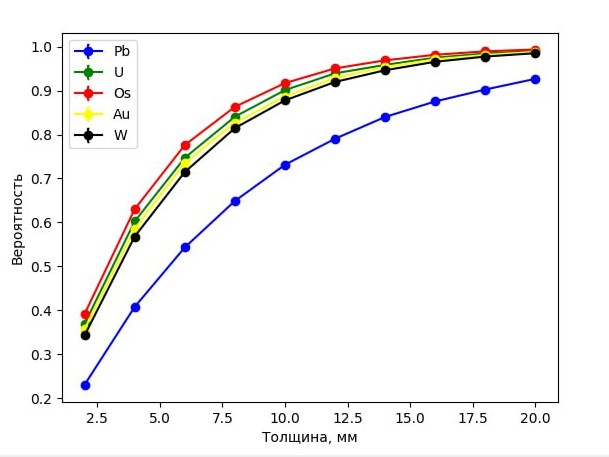
\includegraphics[width=0.7\linewidth]{pictures/fbc984ea-c7c6-41c1-b77b-5bc2c498663d.jpeg}
    \caption{Зависимость вероятности взаимодействия $\gamma-$кванта с энергией 800 МэВ с различными металлами от их толщины. }
    \label{fig:placeholder}
\end{figure}

\section{Обработка данных}
...
\section{Исследование}
В этом разделе изучается эффективность обработки данных при разных параметрах.
\subsection{Зависимость от разброса}
\begin{figure}[H]
    \centering
    \begin{minipage}{0.4\linewidth}
        \centering
        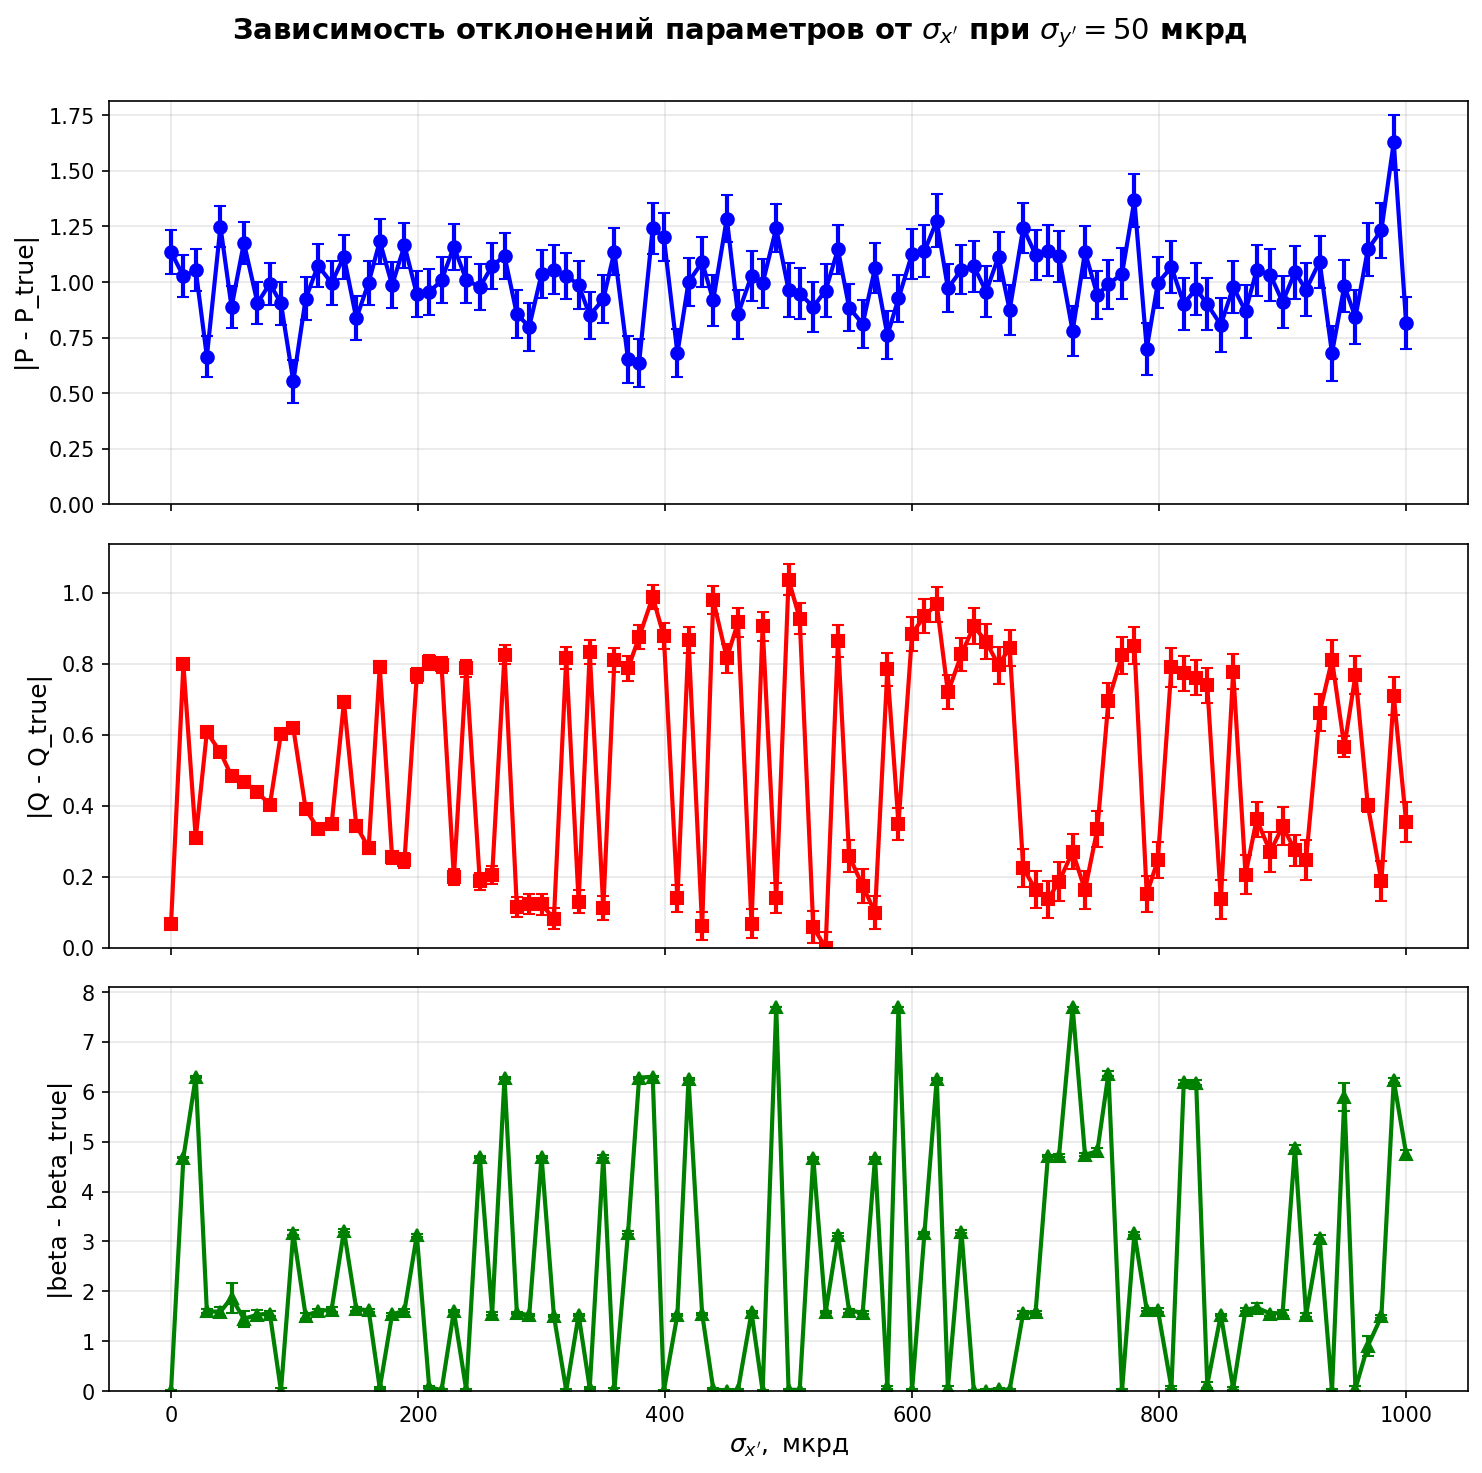
\includegraphics[width=\linewidth]{pictures/gr_2.png}
    \end{minipage}
    \begin{minipage}{0.4\linewidth}
        \centering
        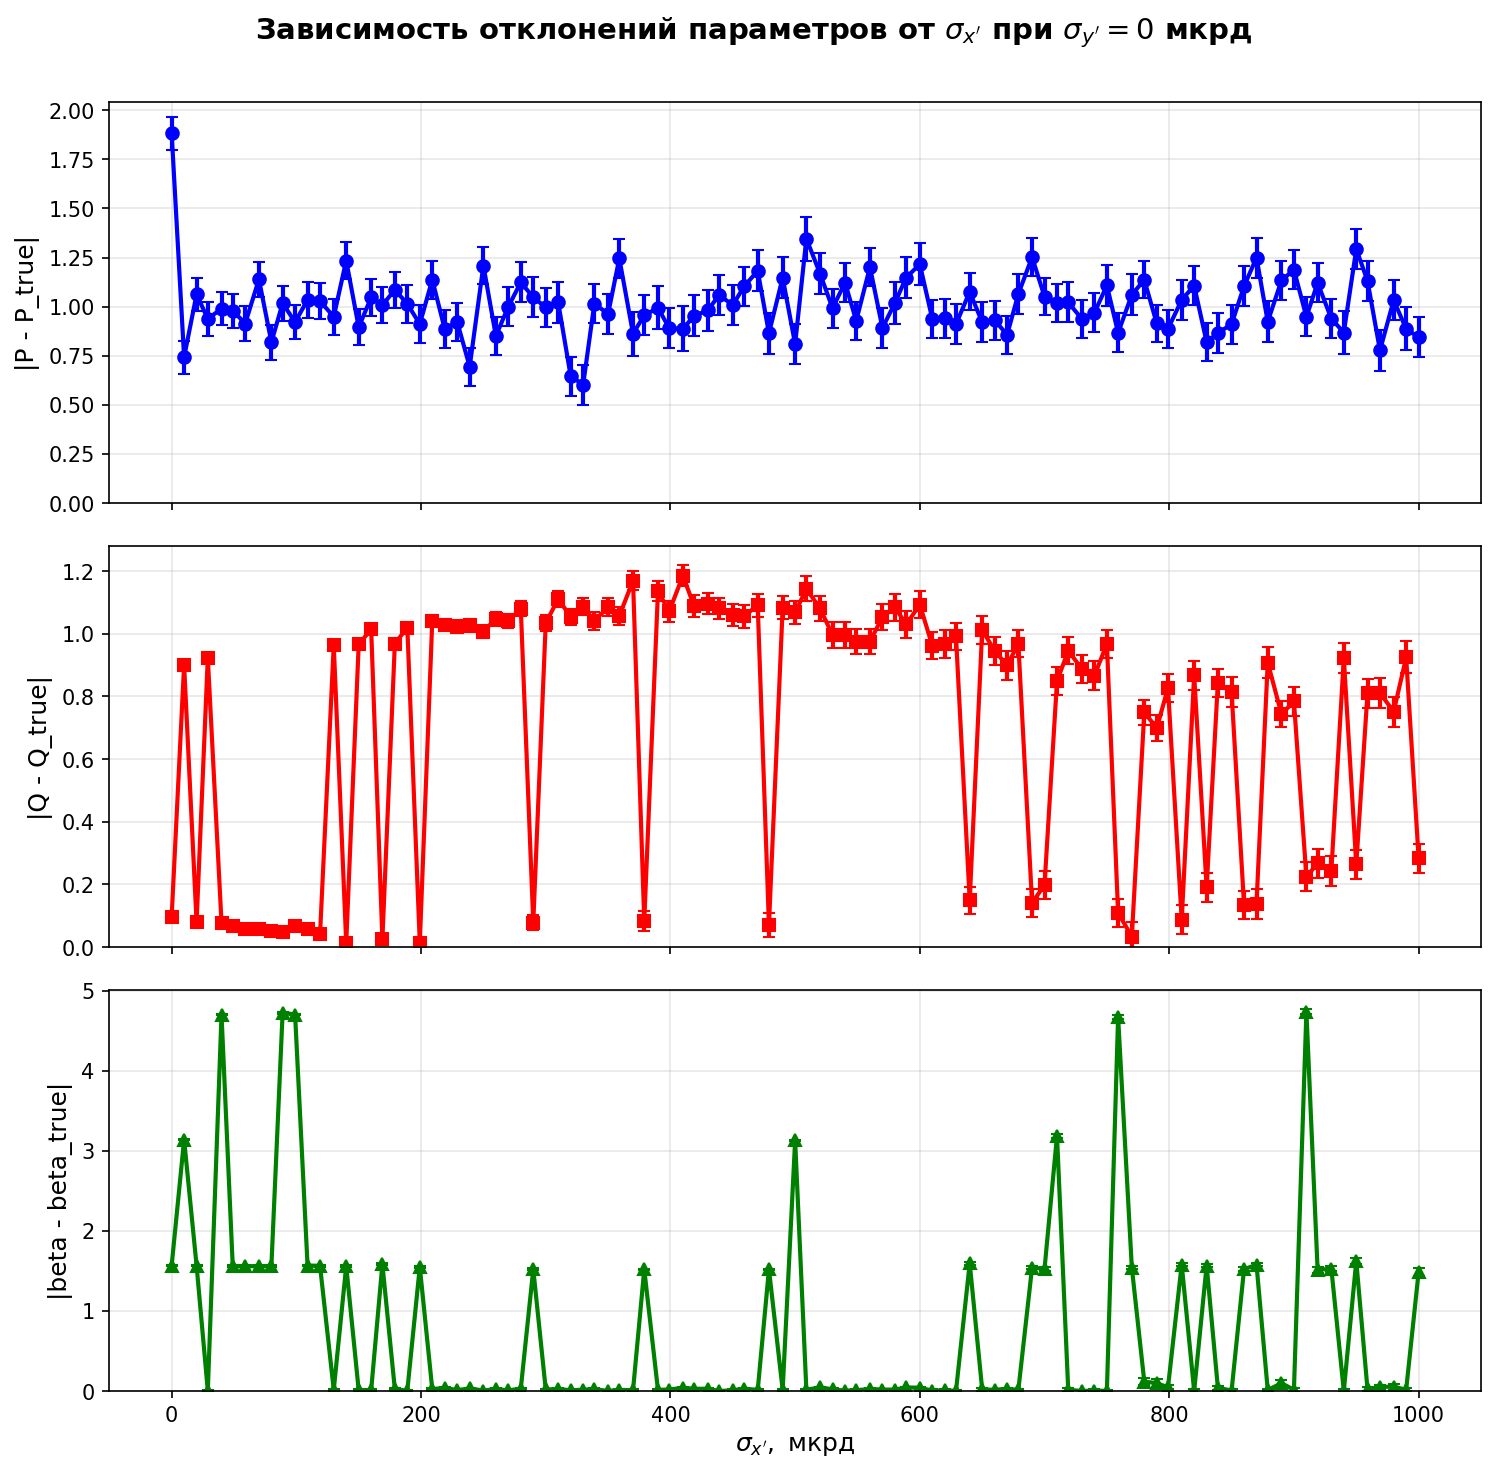
\includegraphics[width=\linewidth]{pictures/gr_3.png}
    \end{minipage}
\end{figure}

\begin{figure}[H]
    \centering
    \begin{minipage}{0.4\linewidth}
        \centering
        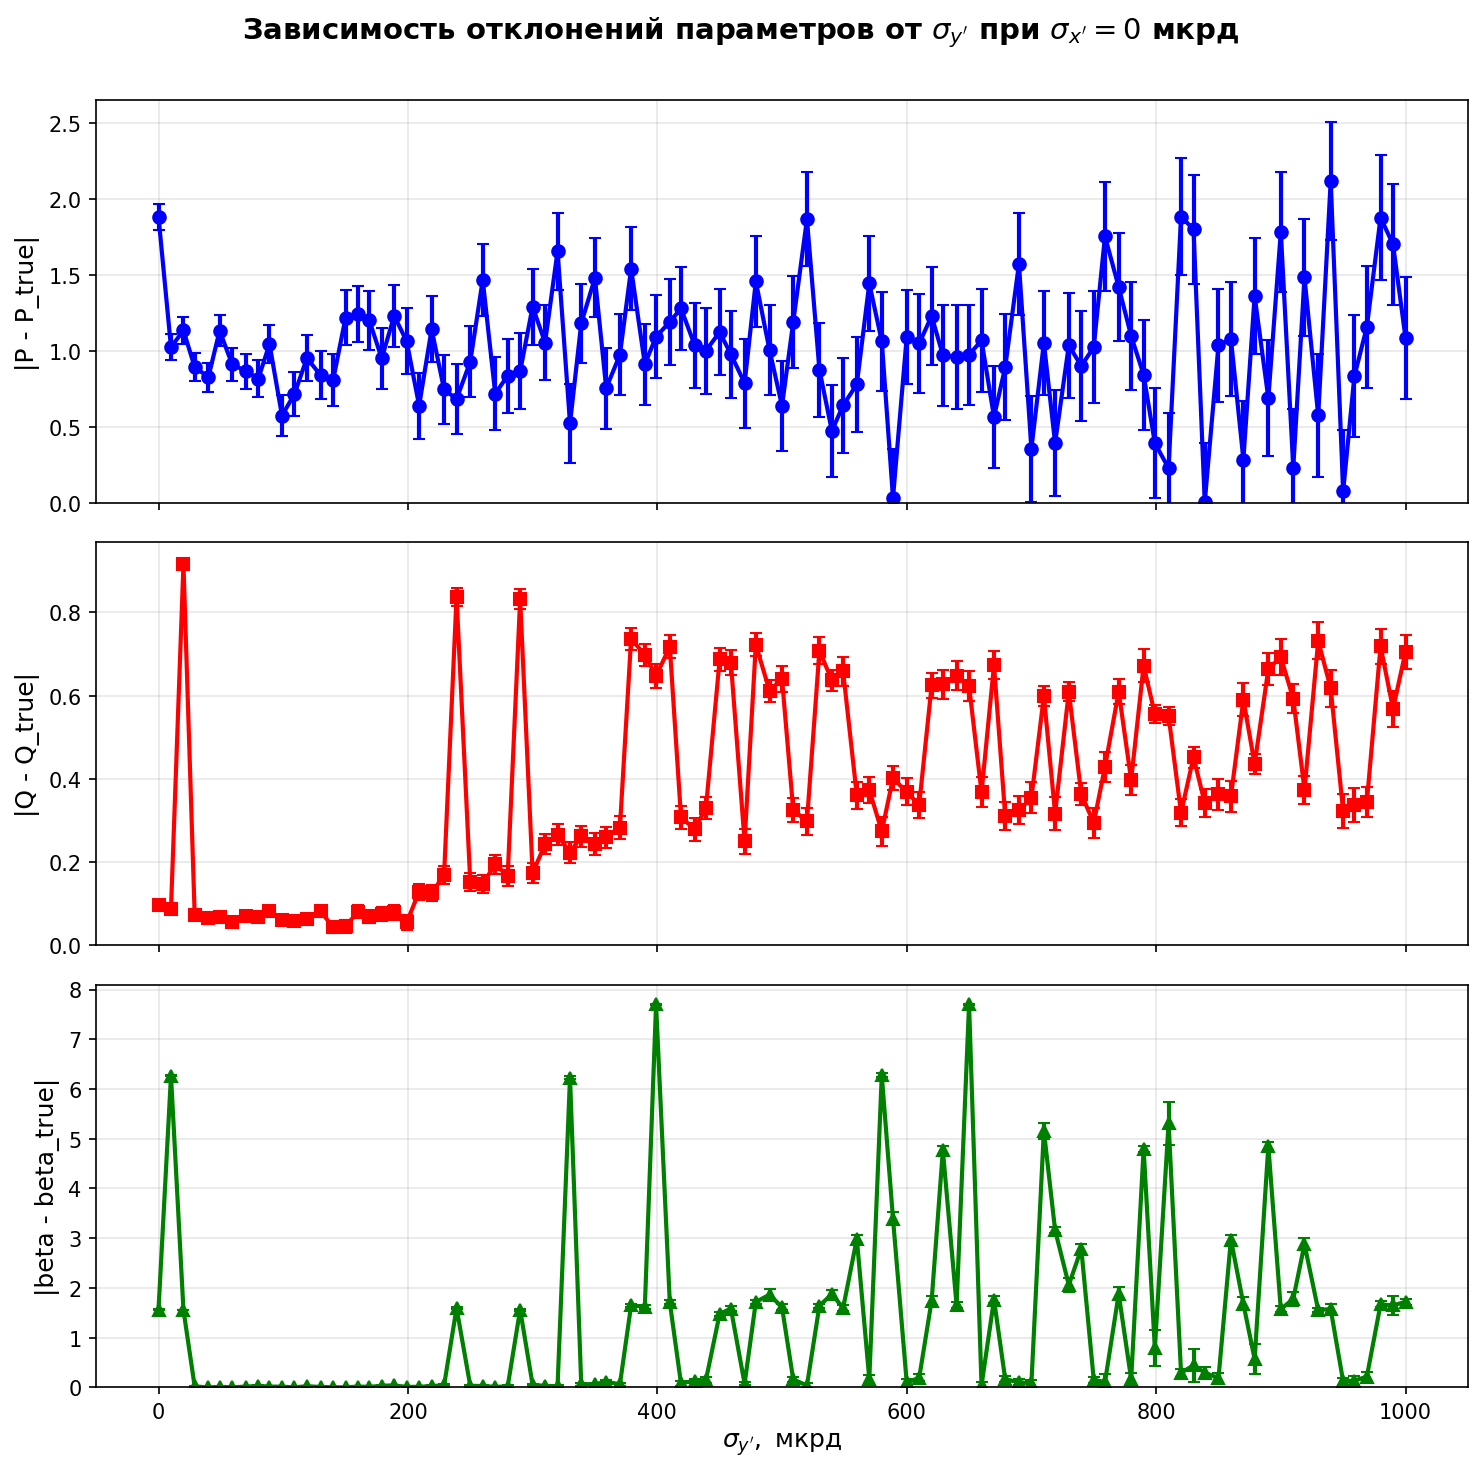
\includegraphics[width=\linewidth]{pictures/gr_4.png}
    \end{minipage}
    \begin{minipage}{0.4\linewidth}
        \centering
        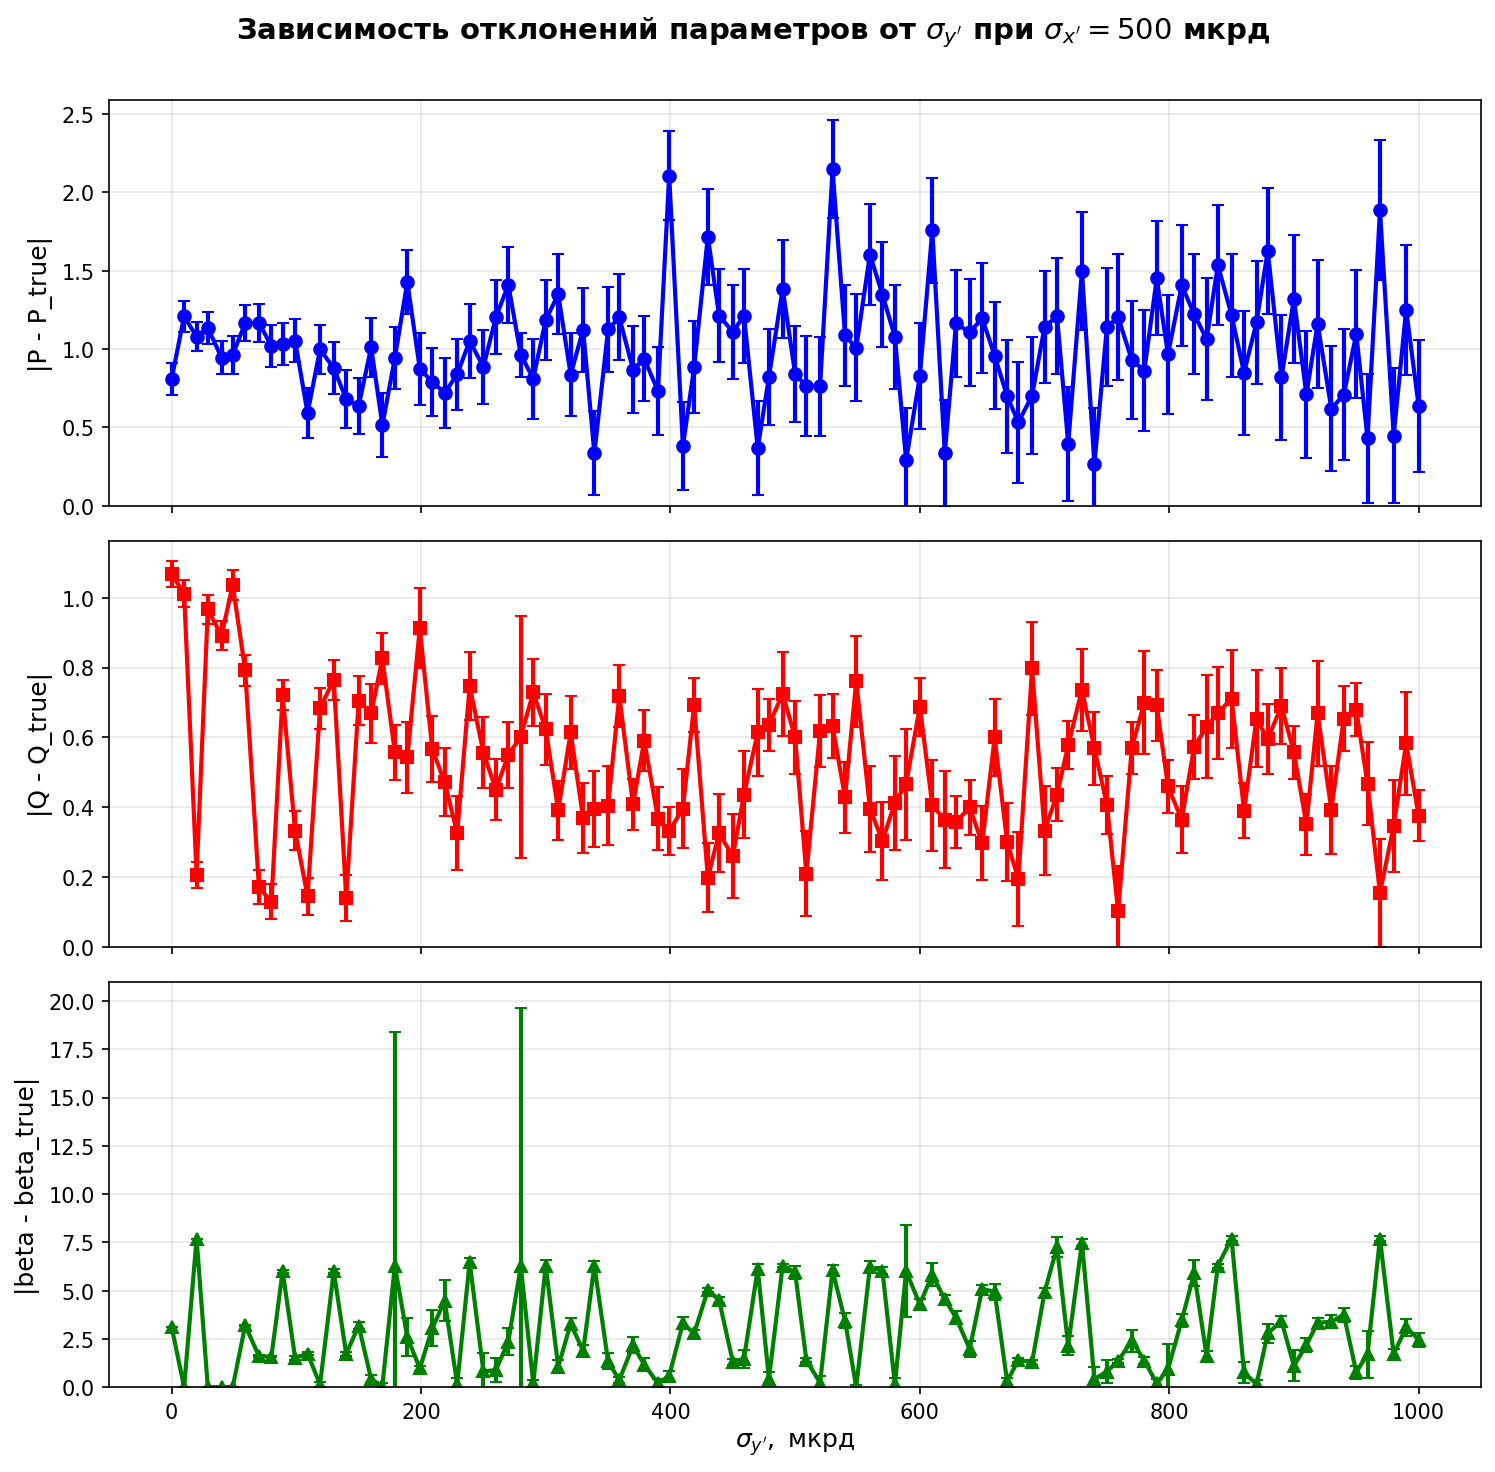
\includegraphics[width=\linewidth]{pictures/gr.png}
    \end{minipage}
\end{figure}

Зависимости подгонки от разброса нет, на выходе мы видим только шум.

\section{Зависимость от параметров}

\section{Подгонка без вещества}

...
\end{document}
